\documentclass[12pt]{article}

\usepackage[margin=1in, paperwidth=8.5in, paperheight=11in]{geometry}
\usepackage[table,xcdraw]{xcolor}
\usepackage{graphicx}
\usepackage{amsmath}
\usepackage{sidecap}
\usepackage{caption}
\usepackage{subcaption}
\usepackage[table,xcdraw]{xcolor}

\begin{document}
\begin{center}
Jeffrey Rodriguez 110733867\\AMS 326\\Report 4\\4/20/2018\\

\end{center}
\section*{4.1}
260 trading days ago, Mr. Poor invests \$1,000,000, with the change rate $X$, for his portfolio following a normal distribution. We wish to see how much money he makes (or loses), given the mean and standard deviation of the random variable $X$.
\\First, we generate 2 random numbers of the form $y_{i+1} =(y_i + y_{i-1})\mod1$, and perform a Box-Muller Transformation to convert them to numbers which follow a standard normal distribution. 260 of these numbers are kept, and then transformed to either $X\sim N(0.1949\%,0.2018\%^2)$, or $X\sim N(-0.1989\%,0.0640\%^2)$ depending on the part of them problem. This transform is done taking the standard normally distributed numbers, $Z$, and defining a new collection of numbers as $X_i = Z_i\cdot\sigma+\mu$.
\\After each day, Mr. Poor will gain or lose money. If he gains (when $s_i > 0$), he will have to pay a fee of 3.333\%.
If he loses money, or has no loss/return, he does not pay a fee, nor receive anything. 
\\Let $V_i$ denote the value on the $i^{\text{th}}$ day. For day 1, the amount is 1,000,000. On each successive day, his new value is $V_{i+1} = V_i(1 + s_i)$. Once all of these values are calculated, for both distributions, we want to look at the total amount Mr. Poor has on the 260$^\text{th}$ day, and plot a time series plot for each day. 
\\Below are the resulting time series plots, side-by-side:
%\begin{figure}[h]
%	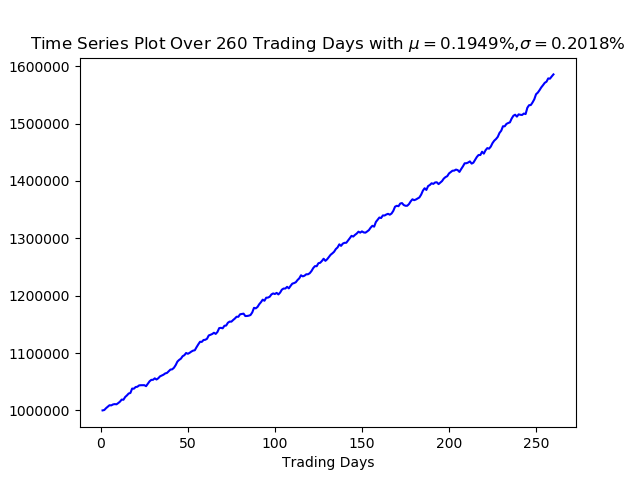
\includegraphics[scale=.5]{11plot.png}
%\end{figure}
%\\The time series plot for the distribution $X\sim N(-0.1989\%,0.0640\%^2)$ is:
%\newpage
%\begin{figure}[h]
%	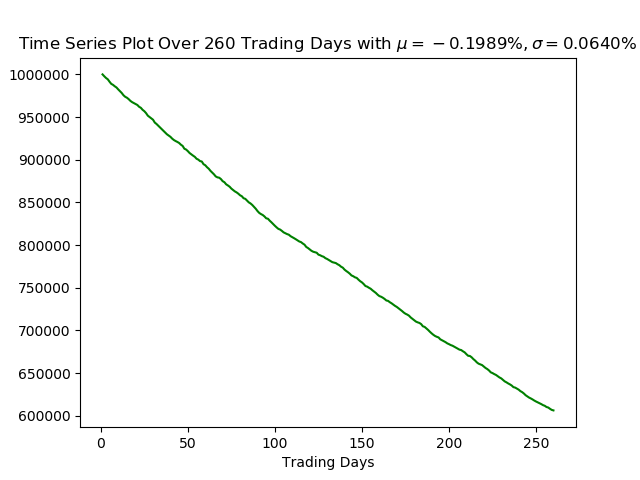
\includegraphics[scale=.5]{12plot.png}
%\end{figure}
\begin{figure}[h]
	\centering
	\begin{subfigure}{.5\textwidth}
		\centering
		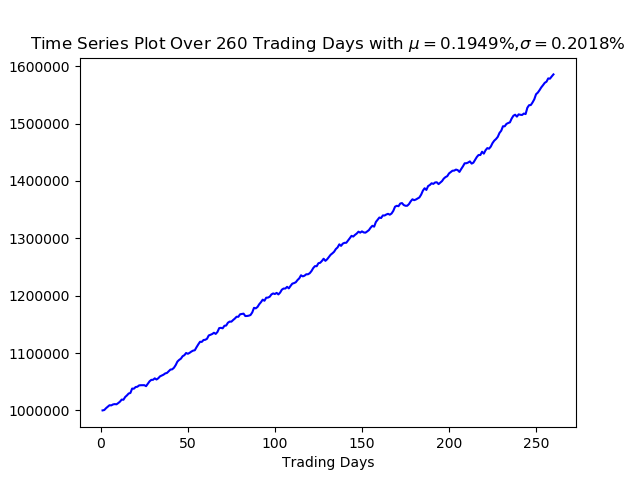
\includegraphics[width=.9\linewidth]{11plot}
		\caption{$X\sim N(0.1949\%,0.2018\%^2)$}
		\label{fig:sub1}
	\end{subfigure}%
	\begin{subfigure}{.5\textwidth}
		\centering
		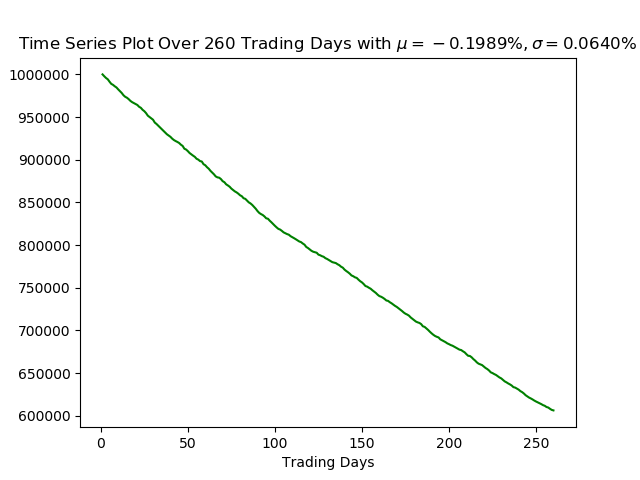
\includegraphics[width=.9\linewidth]{12plot}
		\caption{$X\sim N(-0.1989\%,0.0640\%^2)$}
		\label{fig:sub2}
	\end{subfigure}

	\label{fig:test}
\end{figure}

\newpage
Next is a plot of the two series together:
\begin{figure}[h]
	\centering
	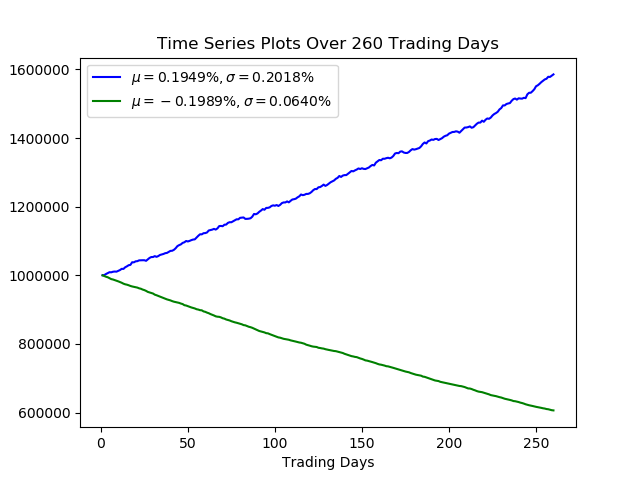
\includegraphics[scale=.75]{13plot.png}
\end{figure}
\\As expected, the line with positive $\mu$ is increasing, and the one with negative $\mu$ is decreasing. Furthermore, the second curve, with smaller standard deviation (and thus variance) $\sigma$ has a change which appears more steady and smooth. On the other hand, the series with higher standard deviation has a more rough appearance with easier to spot changes in increase/decrease. Furthermore, we see that both, respective, have an increase/decrease of roughly \$600,000.
\\The final values are \$1,585,602.53 and \$606,221.19.
\\The code used for plotting and computations can be seen in the file, '326HW4-1.py'.

\newpage
\section*{4.2}
The second problem is a modification of Buffon's Needle, where instead of dropping needles inbetween parallel lines, we use equilateral triangles. $N=$ 300,000,000 trials will be performed, and with this large number, we can compute the probability of a triangle falling on one of the lines. In the case of a triangle of radius $\frac{1}{2}$, with line spacing = 1, the probability of an equilateral triangle crossing over a line is equal to $\frac{3\sqrt{3}}{pi}\approx0.82699$. 
\\First, a centroid for a triangle is generated at the origin. The position of the top vertex directly along the y-axis is defined as $A = (0,\frac{l}{\sqrt{3}})$, with $l$, the side length equal to $\frac{1}{2}$. To generate the other two points of the triangle, we define the rotation matrix: $$T_{\theta}=\begin{pmatrix}
\cos\theta&&-\sin\theta\\\sin\theta&&\cos\theta
\end{pmatrix}$$
\\The bottom left point is positioned at $T_\theta\cdot A$, with $\theta = \frac{2\pi}{3}$. For the bottom right point, we do the same, but use $\theta = \frac{4\pi}{3}$ instead. With this generic triangle created, we can then start the simulation. 
\\To do this, we first generate a center coordinate for the triangle to be shifted over by, and generate an arbitrary angle $\theta\in[0,2\pi]$. Let $A' = T_\theta\cdot A$. Note that $A_x = 0$, so $A' = <A_y\sin\theta, A_y\cos\theta>$.
The $y$ components for $B',~C'$ are generated by performing $T_\theta\cdot A'$, with $\theta$ as the same set of  values used to generate the original triangle. However, to minimize computation time, we only use the equation of the $y$ component. 
\\So, $B_y' = A_x'\sin\frac{2\pi}{3} + A_y'\cos\frac{2\pi}{3}$, and $C_y' = B_y' = A_x'\sin\frac{4\pi}{3} + A_y'\cos\frac{4\pi}{3}$. After transforming these points, they are then shifted by the center coordinate previously generated.
If $A_y', ~B_y',$ or $C_y'$ is less than 0, or greater than 1, we know that the triangle has crossed a line and can increment a counter. This is done via a loop of range($N$=300,000,000). We find this to be roughly 0.4348.
\\The code used for this can be seen in the file, 'MCTriangle.java'.
\newpage
\section*{4.3}
The third problem gives us a set of conditions for a boat traveling across a river, and asks us to compute its trajectory as its position along the x-axis changes. Wind must also be accounted for, and is represented as $w(x) = 4v_0(\frac{x}{a} - (\frac{x}{a})^2)$, where $(a,0)$ denotes the starting position of the boat.
\\We model this as the system of ODEs defined as $$y'(t) = w(x) - v_B\sin\theta = w(x) - v_B \frac{y}{\sqrt{x^2+y^2}}$$
\\$$x'(t)=v_B\cos\theta = v_B\frac{x}{\sqrt{x^2+y^2}}$$
\\A two dimensional Runge-Kutta method is implemented on this, with values $k_i,~l_i$ defined as: $k_1 = f(t_i,x_i,y_i),~ l_1 = g(t_i,x_i,y_i)
\\k_2 = f(t_i + \frac{1}{2}\Delta t, x_i + \frac{1}{2}\Delta t k_1 ,y_i + \frac{1}{2}\Delta t l_1),~ l_2 = g(t_i + \frac{1}{2}\Delta t, x_i + \frac{1}{2}\Delta t k_1 ,y_i + \frac{1}{2}\Delta t l_1)
\\k_3 = f(t_i + \frac{1}{2}\Delta t, x_i + \frac{1}{2}\Delta t k_2 ,y_i + \frac{1}{2}\Delta t l_2),~ l_3 = g(t_i + \frac{1}{2}\Delta t, x_i + \frac{1}{2}\Delta t k_2,y_i + \frac{1}{2}\Delta t l_2)
\\k_4 = f(t_i +\Delta t, x_i + \Delta t k_3, y_i + \Delta t l_3),~l_4 = g(t_i + \Delta t, x_i + \Delta t k_3, y_i + \Delta t l_3)
\\k = \frac{1}{6}(k_1 + 2(k_2 + k_3) + k_4),~
l = \frac{1}{6}(l_1 + 2(l_2 + l_3) + l_4)$
\\with $t_{i+1} = t_i + \Delta t,~ x_{i+1} = x_i + \Delta t k,~ y_{i+1} = y_i + \Delta t l$. This is iterated $n = a / h = 1000/0.001 = 1,000,000$ times.
The initial conditions are $y(x = a) = 0$, $y(x = 0) = 0$, with $a = 1000$ and $v_0 = 10$. The Runge-Kutta method is performed for $v_B = 5, 10, 15$ giving maximum $y$ values of 1345.87, 345.43, and 210.30 respectively. Following is a graph for these three $v_B$ conditions. 
\begin{figure}[h]
	\centering
	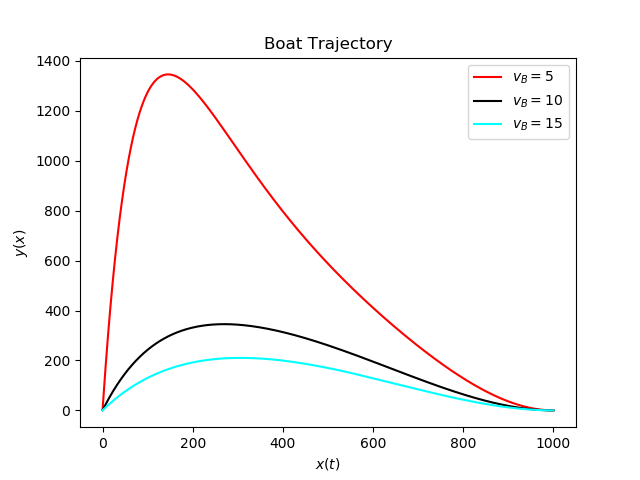
\includegraphics[scale=.5]{3plot.png}
\end{figure}
\\The code used for plotting and computations can be seen in the file, '326HW4-3.py'.
\end{document}